% Show distributions for loose cuts, 5e19 data/MC comparison
% Aggressive cuts, 6.6e20 Projection
% Current efficiency and purity plots as a function of energy

\section{Electron-Like Event Distributions}\label{sec:electron_like}
\subsection{Reconstructed energy spectrum}
The reconstructed energy spectrum of the selected events after the application of the background-rejection cuts is shown in Figure \ref{fig:spectrum_after}. It corresponds to the sum of the reconstructed energies of the shower-like objects, as described in Section \ref{sec:showerenergy}, and the reconstructed energies of the track-like objects, as described in Section \ref{sec:protonenergy}. 

\begin{figure}[htbp]
\centering
  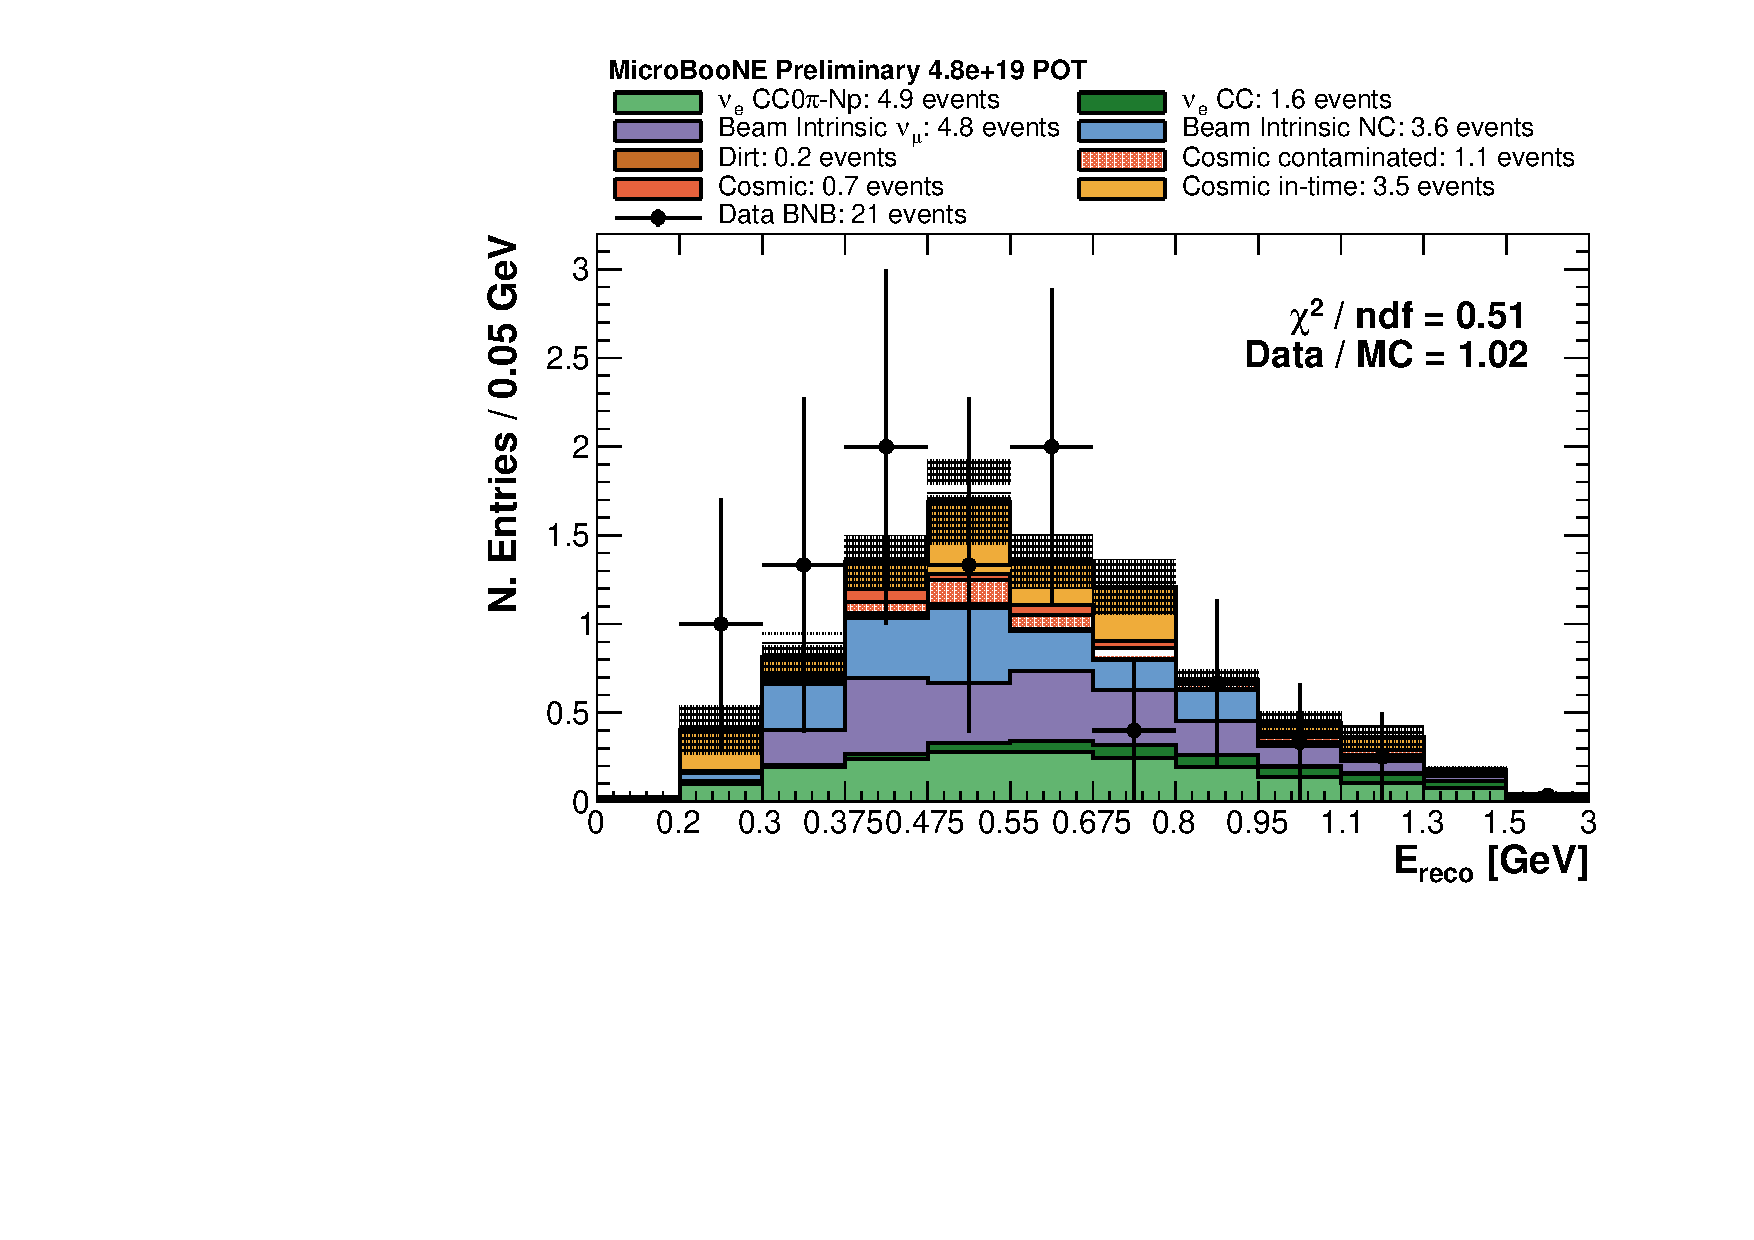
\includegraphics[width=0.65\linewidth]{figures/h_fixed_energy_after.pdf}
    \caption{Reconstructed energy spectrum of the selected events after the background-rejection cuts.}\label{fig:spectrum_after}

\end{figure}


The final number of selected data events in the unblinded data sample is 21, corresponding to a MicroBooNE exposure of \num{4.84e19} POT. These events have been hand-scanned: Figure \ref{fig:evds} shows the event displays of two $\nu_{e}$-like selected data events.


The data BNB distribution is in good agreement with the stacked Monte Carlo + EXT distributions, both in normalization (the integral ratio is 1.03) and in shape ($\chi^2 /\mathrm{n.d.f.} = 0.68$). 
%The signal component ($\nu_{e}$ CC0$\pi$-Np events) represents now the largest component among the event categories with 4.1 events. 

\subsection{Efficiency and purity}
It is now possible to calculate the efficiency and the purity of our $\nu_{e}$ CC0$\pi$-Np selection after the background-rejection cuts, as defined in Section \ref{sec:eff}. The background-rejection cuts were aimed to improve the significance of the $\nu_{e}$ CC0$\pi$-Np events in our sample. Thus, the efficiency decreases, from 41.1\% to 14.3\%, since the cuts will eventually remove also some signal events, but the purity increases by a factor of $\sim50$, from 0.5\% to 23.9\%. Figure \ref{fig:effafter} shows the efficiency as a function of the true neutrino energy and the purity as a function of the reconstructed energy, before and after the background rejection cuts. 

\begin{figure}
  \begin{subfigure}{0.48\textwidth}
    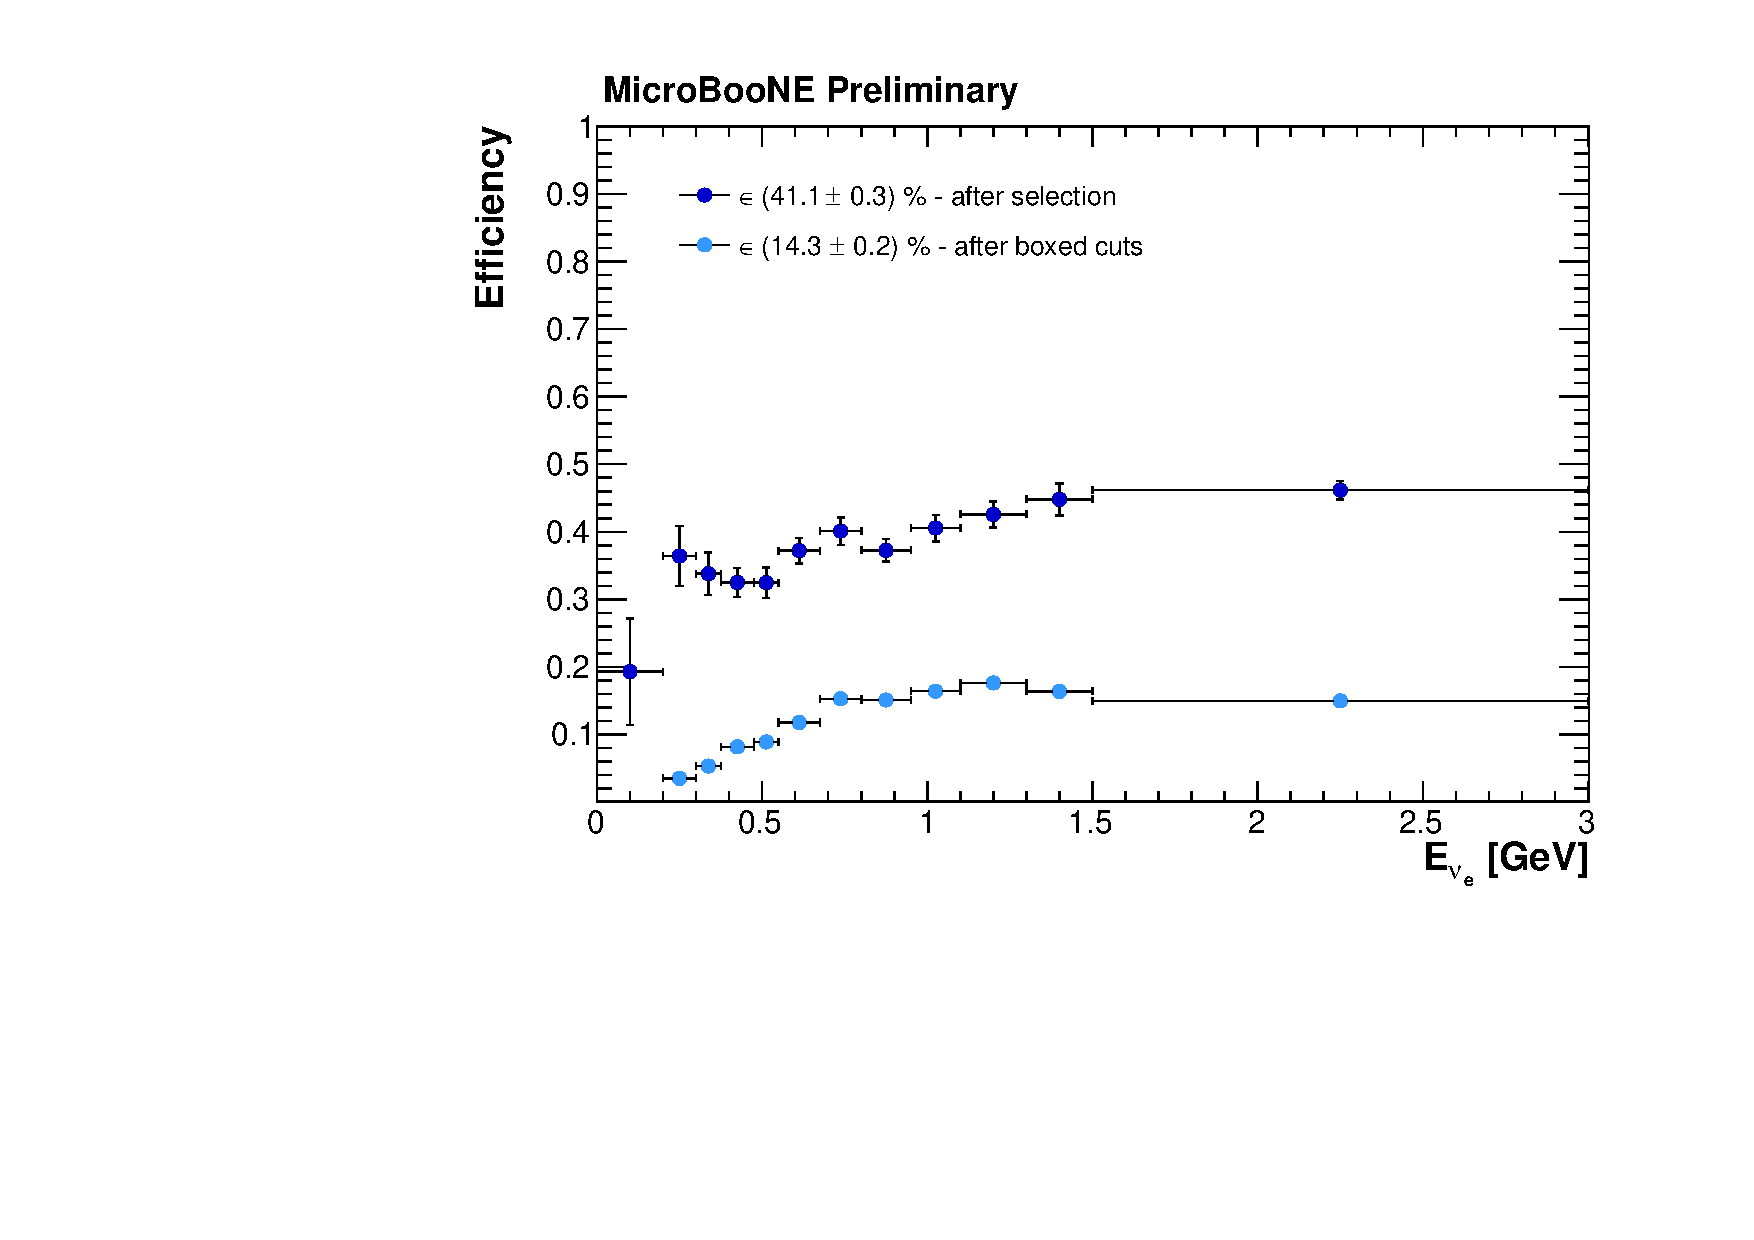
\includegraphics[width=\linewidth]{figures/eff_after.pdf}
    \caption{Efficiency} 
  \end{subfigure}
    \begin{subfigure}{0.48\textwidth}
    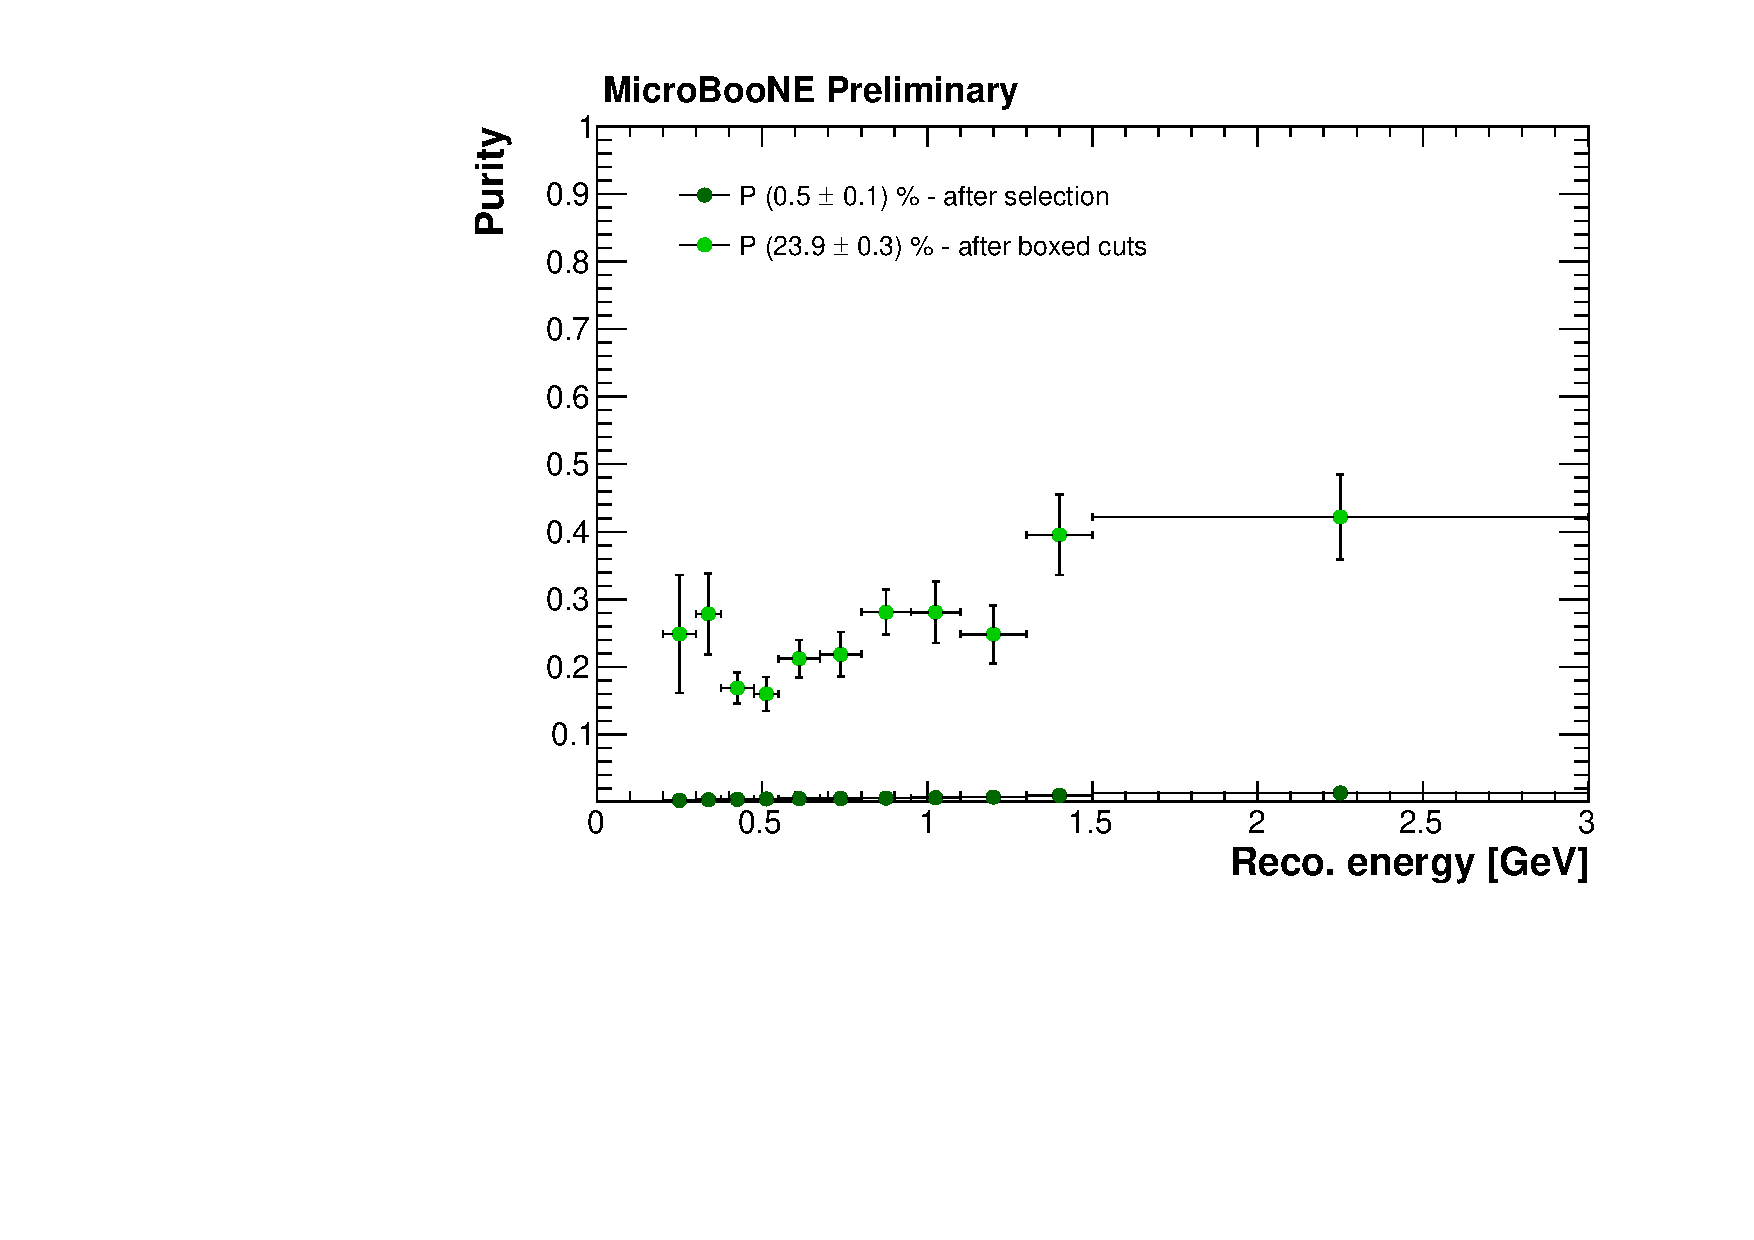
\includegraphics[width=\linewidth]{figures/purity_after.pdf}
    \caption{Purity} 
  \end{subfigure}
  \caption{Left: $\nu_{e}$ CC$0\pi$-Np reconstruction efficiency as a function of the true $\nu_{e}$ energy before and after the background-rejection cuts. Right: $\nu_{e}$ CC$0\pi$-Np purity as a function of the reconstructed energy before and after the background-rejection cuts.}
  \label{fig:effafter}
\end{figure}

Table \ref{tab:effafter} shows the efficiency and the number of events selected for each event category before and after the background-rejection cuts. In particular, we are able to reject the 99.5\% of the neutrino background and the 
99.996\% of the cosmogenic background, while retaining a 14.3\% $\nu_{e}$ CC0$\pi$-Np efficiency.

\begin{table}[htbp]
   \centering
   \begin{tabular}{llrrrrrrrr}
     \toprule
     Category & \phantom{a} & Generated & \phantom{a} & Selected & \phantom{a} & After cuts & \phantom{a} & Efficiency\\
     \midrule

     $\nu_{e}$ CC0$\pi$-Np       & & 34.8     & & 14.3   & & 4.9   & & 14.3\%\\
     $\nu_{e}$ CC                & & 35.7     & & 13.2   & & 1.6   & & 4.5\%\\
     Beam intrinsic $\nu_{\mu}$  & & 11337.4  & & 918.3  & & 5.0   & & 0.044\%\\
     Beam intrinsic NC           & & 3633.9   & & 342.2  & & 3.3   & & 0.09\%\\
     Dirt                        & & 2609.5   & & 37.1   & & 0.3   & & 0.01\%\\
     Cosmic in-time              & & 135377.2 & & 1151.6 & & 3.5   & & 0.003\%\\
     Cosmic contaminated         & & -        & & 260.7  & & 1.1   & & 0.4\%\\
     Cosmic                      & & -        & & 233.3  & & 0.9   & & 0.4\%\\

     \bottomrule
   \end{tabular}
   \caption{Summary of the selection algorithm results, showing the contribution of each event category, for a MicroBooNE exposure of \num{4.84e19} POT.}\label{tab:effafter}
\end{table}

\begin{figure}[htbp]
\centering
  \begin{subfigure}{0.7\textwidth}
  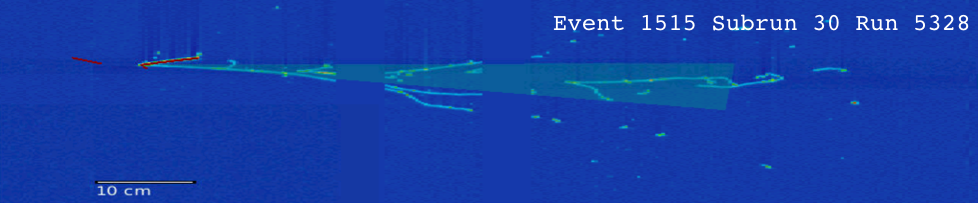
\includegraphics[width=\linewidth]{figures/data1.png}
    \caption{Event 1515, Subrun 30, Run 5328}
\end{subfigure}
  \begin{subfigure}{0.7\textwidth}	
  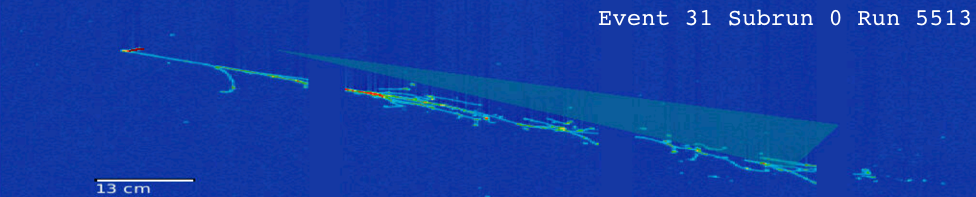
\includegraphics[width=\linewidth]{figures/data2.png}
  \caption{Event 31, Subrun 0, Run 5513}
\end{subfigure}

  \caption{Event displays of the collection plane of two $\nu_{e}$-like data events present in our sample after the background-rejection cuts. The gaps are caused by the presence of missing or unresponsive wires. The red lines correspond to reconstructed track-like objects and the green cones correspond to reconstructed shower-like objects. }
  \label{fig:evds}
\end{figure}